%%%%%%%%%%%%%%%%%%%%%%%%%%%%%%%%%%%%%%%%%
% Beamer Presentation
% LaTeX Template
% Version 1.0 (10/11/12)
%
% This template has been downloaded from:
% http://www.LaTeXTemplates.com
%
% License:
% CC BY-NC-SA 3.0 (http://creativecommons.org/licenses/by-nc-sa/3.0/)
%
%%%%%%%%%%%%%%%%%%%%%%%%%%%%%%%%%%%%%%%%%

%----------------------------------------------------------------------------------------
%	PACKAGES AND THEMES
%----------------------------------------------------------------------------------------

\documentclass[8pt,sans,mathserif]{beamer}%aspectratio=43

\usepackage{ucs}
\usepackage[T1]{fontenc}
\usepackage[utf8x]{inputenc}
\usepackage[english, greek]{babel}
%\usepackage{kerkis}

%\hypersetup{pdfpagemode=FullScreen}
\usepackage{multimedia}
%\usepackage{movie15}
\usepackage{hyperref}

\mode<presentation> {

% The Beamer class comes with a number of default slide themes
% which change the colors and layouts of slides. Below this is a list
% of all the themes, uncomment each in turn to see what they look like.

%\usetheme{default}
%\usetheme{AnnArbor}
%\usetheme{Antibes}%good
%\usetheme{Bergen}
%\usetheme{Berkeley}
%\usetheme{Berlin}
%\usetheme{Boadilla}
%\usetheme{CambridgeUS}%good red
%\usetheme{Copenhagen}
\usetheme{Darmstadt}%good margin
%\usetheme{Dresden}
%\usetheme{Frankfurt}
%\usetheme{Goettingen}
%\usetheme{Hannover}
%\usetheme{Ilmenau}
%\usetheme{JuanLesPins}%good
%\usetheme{Luebeck}
%\usetheme{Madrid}
%\usetheme{Malmoe}
%\usetheme{Marburg}
%\usetheme{Montpellier}
%\usetheme{PaloAlto}
%\usetheme{Pittsburgh}
%\usetheme{Rochester}
%\usetheme{Singapore}
%\usetheme{Szeged}
%\usetheme{Warsaw}

% As well as themes, the Beamer class has a number of color themes
% for any slide theme. Uncomment each of these in turn to see how it
% changes the colors of your current slide theme.

%\usecolortheme{albatross}
%\usecolortheme{beaver}
%\usecolortheme{beetle}
%\usecolortheme{crane}
%\usecolortheme{dolphin}
%\usecolortheme{dove}
%\usecolortheme{fly}
%\usecolortheme{lily}
%\usecolortheme{orchid}
%\usecolortheme{rose}
%\usecolortheme{seagull}
%\usecolortheme{seahorse}
%\usecolortheme{whale}
%\usecolortheme{wolverine}

%\setbeamertemplate{footline} % To remove the footer line in all slides uncomment this line
%\setbeamertemplate{footline}[page number] % To replace the footer line in all slides with a simple slide count uncomment this line

\setbeamertemplate{navigation symbols}{} % To remove the navigation symbols from the bottom of all slides uncomment this line
}

\usepackage{graphicx} % Allows including images
\usepackage{booktabs} % Allows the use of \toprule, \midrule and \bottomrule in tables

% New commands-environments
\newcommand{\eng}[1]{\selectlanguage{english}#1\selectlanguage{greek}}
\newcommand{\gre}[1]{\selectlanguage{greek}#1\selectlanguage{english}}

\newcommand{\norm}[1]{\left\lVert#1\right\rVert}

%----------------------------------------------------------------------------------------
%	TITLE PAGE
%----------------------------------------------------------------------------------------

\title[Καταγραφή και Δυναμική Ανάλυση της Κίνησης του Ανθρώπου]{Καταγραφή και Δυναμική Ανάλυση της Κίνησης του Ανθρώπου}

%\author{\eng{Stanev Dimitar}} % Your name
\institute[ΗΜ\&ΤΥ]{
{\large\textsc{Πανεπιστήμιο Πατρών \\
Τμήμα Ηλεκτρολόγων Μηχανικών και Τεχνολογίας Υπολογιστών}}\\[1cm]
{\large\eng{Stanev Dimitar}}\\
\medskip
\textit{\eng{jimstanev@gmail.com}} % Your email address
}
\date{\today} % Date, can be changed to a custom date

\begin{document}

\logo{
\includegraphics[height=1cm]{fig/university-patras.jpg}}%logo

\begin{frame}
\titlepage % Print the title page as the first slide
\end{frame}

%----------------------------------------------------------------------------------------
%	PRESENTATION SLIDES
%----------------------------------------------------------------------------------------

%\begin{frame}
%\frametitle{Test}
%
%    \begin{center}
%        \movie[start=6s, width=11cm,height=6cm, poster]{}{video/filter0.avi}
%    \end{center}
%\end{frame}

%\begin{frame}
%    \begin{block}{Test}
%        \includemovie[autoplay, poster]{4cm}{3cm}{video/filter0.avi}
%    \end{block}
%\end{frame}

%%%%%%%%%%%%%%%%%%%%%%%%%%%%%%%%%%%%%%%%%%%%%%%%%%%%%%%%%%%%%%%%%%%%%%%%%%%%%%%%
\section{Εισαγωγή}
\frame{\tableofcontents[currentsection]}
\subsection{Περιγραφή της Διπλωματικής Εργασίας}
\begin{frame}
\frametitle{Σκοπός}

    \begin{block}{Σκοπός}
        \begin{itemize}
            \item Ανάπτυξη συστήματος καταγραφής της ανθρώπινης κίνησης
            \item Μοντελοποίηση μυοσκελετικού μοντέλου του ανθρώπου
            \item Δυναμική ανάλυση της καταγεγραμμένης κίνησης (αντίστροφη κινηματική, αντίστροφη δυναμική, ορθή δυναμική, υπολογισμός μυϊκών διεγέρσεων)
        \end{itemize}
    \end{block}

\end{frame}

\subsection{Ενδεικτικές Εφαρμογές}
\begin{frame}
\frametitle{Κινητήριο παράδειγμα}

    \begin{figure}[c]
        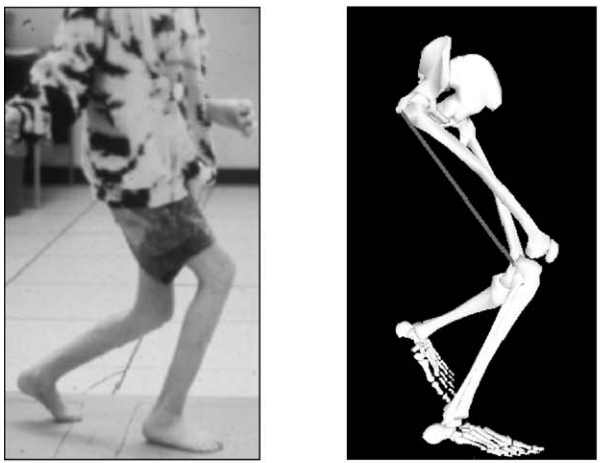
\includegraphics[height=0.8\textheight, keepaspectratio]{fig/crouch-gait.png}
    \end{figure}

    \onslide<1->\let\thefootnote\relax\footnote{\hspace{-12pt}\eng{Arnolda A., "The role of estimating muscle-tendon lengths and velocities of the hamstrings in the evaluation and treatment of crouch gait", 2006}}

\end{frame}

%%%%%%%%%%%%%%%%%%%%%%%%%%%%%%%%%%%%%%%%%%%%%%%%%%%%%%%%%%%%%%%%%%%%%%%%%%%%%%%%
\section{Καταγραφή της Κίνησης}
\frame{\tableofcontents[currentsection]}

\subsection{Η Συσκευή Ανίχνευσης}
\begin{frame}
\frametitle{Χαρακτηριστικά της συσκευής \eng{Kinect}}

    \begin{columns}
    \column{0.5\textwidth}
        \begin{figure}[c]
            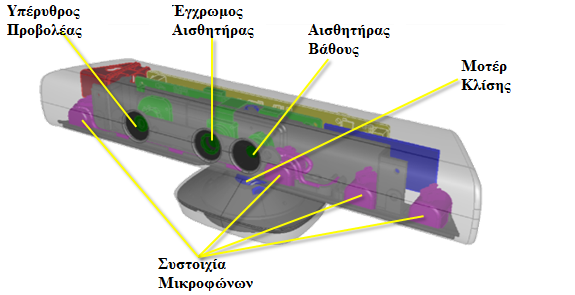
\includegraphics[width=1.0\linewidth, keepaspectratio]{fig/kinect-characteristics.png}
        \end{figure}

        \pause

        \column{0.5\textwidth}
        \begin{figure}[c]
            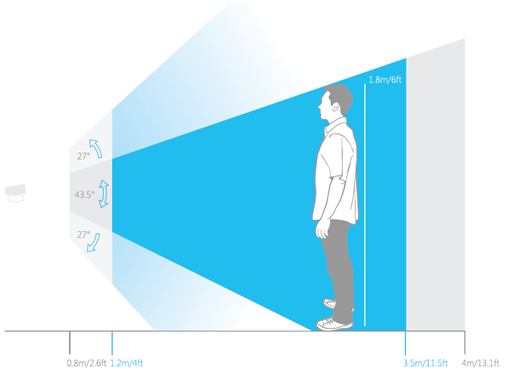
\includegraphics[width=1.0\linewidth, keepaspectratio]{fig/kinect-operation-mode.png}
        \end{figure}
    \end{columns}

    \pause

    \begin{center}
        \begin{tabular}{ll}
            \toprule
            % after \\: \hline or \cline{col1-col2} \cline{col3-col4} ...
            \multicolumn{2}{c}{Χαρακτηριστικά} \\
            \midrule
            Ανάλυση & $1280\times 960, \quad 1024\times 768,$ \\
            & $640\times 480, \quad 320\times 240$ \\
            Υπέρυθρη αόρατη δέσμη & $0.4m$ έως $3.5m$ \\
            Χάρτης βάθους, \eng{RGB} ροή δεδομένων & μέχρι 30 \eng{FPS} \\
            Ρύθμιση κάθετης κλίσης & $\pm 27^{o}$ \\
            Κάθετο πεδίο ορατότητας & $43.5^{ο}$ \\
            Οριζόντιο πεδίο ορατότητας & $57^{ο}$ \\
            \bottomrule
        \end{tabular}
    \end{center}

    \onslide<1->\let\thefootnote\relax\footnote{\hspace{-12pt}\eng{\url{http://msdn.microsoft.com/en-us/library/jj131033.aspx}}}

\end{frame}

\subsection{Εναλλακτικά Εργαλεία}
\begin{frame}
\frametitle{\eng{Kinect Microsoft API vs OpenNI}}

    \begin{itemize}
        \item Υποστήριξη λειτουργικού συστήματος
        \item Γλώσσες προγραμματισμού
        \item Βαθμονόμιση συσκευής
        \item Δυνατότητες ανίχνευσης σκελετού
        \item Δομές φίλτρων
    \end{itemize}

    \begin{columns}
        \column<1>{0.4\textwidth}
        \begin{figure}[t]
            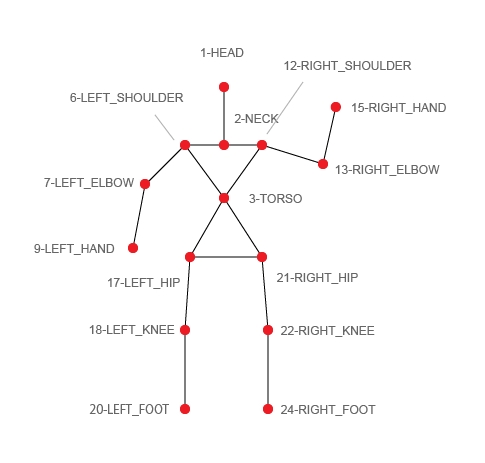
\includegraphics[width=1.0\linewidth, keepaspectratio]{fig/openni-skeleton.png}
        \end{figure}
        \column<1>{0.6\textwidth}
        \begin{figure}[t]
            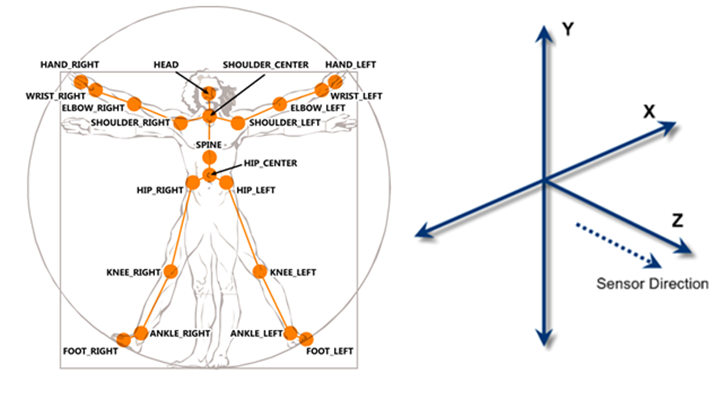
\includegraphics[width=1.0\linewidth, keepaspectratio]{fig/kinect-joints.png}
        \end{figure}
    \end{columns}

\end{frame}

\subsection{Αλγόριθμος Ανίχνευσης Σκελετού}
\begin{frame}
\frametitle{Βασικές αρχές αλγορίθμου}

    \only<1>{
    \begin{figure}[t]
        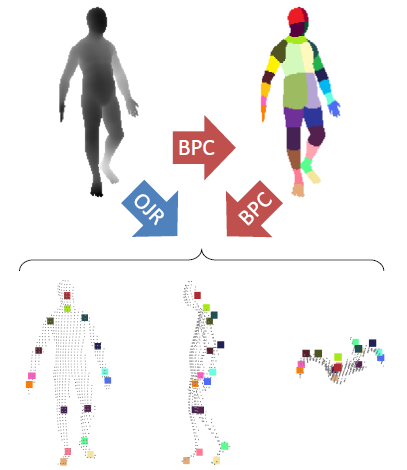
\includegraphics[width=0.6\linewidth, height=0.7\textheight, keepaspectratio]{fig/kinect-algorithms.png}
    \end{figure}

    %\begin{figure}[t]
%        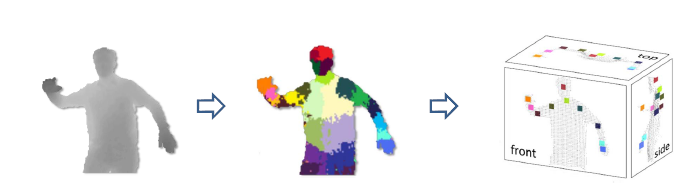
\includegraphics[width=0.8\linewidth, keepaspectratio]{fig/kinect-skeleton-algorithm.png}
%    \end{figure}
    }

    \only<2-3>{
    \begin{columns}
        \column<2-3>{0.5\textwidth}
        \begin{figure}[t]
            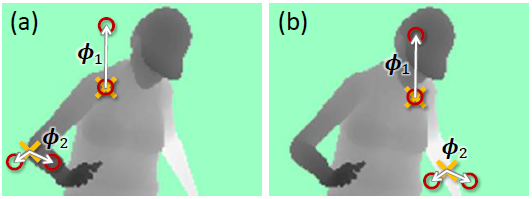
\includegraphics[width=1.0\linewidth, keepaspectratio]{fig/kinect-depth-function.png}
        \end{figure}
        \column<2-3>{0.5\textwidth}
        \begin{equation*}
            f(u|\phi ) = z\big( u + \frac{\delta_1}{z(u)}\big)-z\big( u + \frac{\delta_2}{z(u)}\big)
        \end{equation*}
    \end{columns}

    \begin{columns}
        \column<3>{0.5\textwidth}
        \begin{figure}[t]
            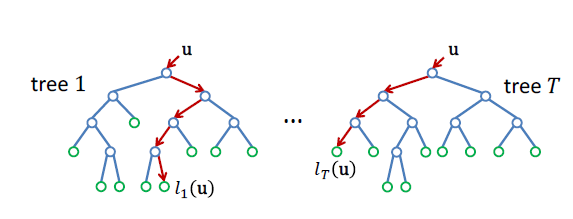
\includegraphics[width=1.0\linewidth, keepaspectratio]{fig/random-decision-forest.png}
        \end{figure}
        \column<3>{0.5\textwidth}
        \begin{equation*}
            p(c|u) = \frac{1}{T} \cdot \sum_{l \in L(u)} p_{l}(c)
        \end{equation*}
    \end{columns}
    }

    \only<4>{
    \begin{block}{Πλεονεκτήματα αλγορίθμου}
        \begin{itemize}
            \item Υπάρχει εσωτερική υλοποίηση
            \item Δεν απαιτεί κάποια ρύθμιση από τον χρήστη
            \item Ταχύτατος (υλοποίηση σε υλικό εσωτερικά)
            \item Καλύπτει μεγάλη ποικιλία ανθρώπων (προσαρμοστικός, αυτοεκπαίδευση)
            \item Μεγάλα ποσοστά ακρίβειας (90\%)
        \end{itemize}
    \end{block}
    }

    \onslide<1-3>\let\thefootnote\relax\footnote{\hspace{-12pt}\eng{Shotton J., "Efficient Human Pose Estimation from Single Depth Images", 2011}}
\end{frame}

\subsection{Θόρυβος}
\begin{frame}
\frametitle{Αντιμετώπιση θορύβου στις μετρήσεις}

    \only<1>{
    \begin{columns}
        \column{0.5\textwidth}
        \begin{figure}[t]
            
\includegraphics[width=0.6\linewidth, keepaspectratio]{fig/hand1.png}
        \end{figure}
        \column{0.5\textwidth}
        \begin{figure}[t]
            
\includegraphics[width=0.6\linewidth, keepaspectratio]{fig/hand2.png}
        \end{figure}
    \end{columns}

    \begin{block}{Κριτήρια Φιλτραρίσματος}
        \begin{itemize}
            \item Την φύση της κίνησης (ταχύτητα)
            \item Εισαγωγή καθυστέρησης λόγω φιλτραρίσματος
            \item Εφαρμογή πραγματικού ή μη πραγματικού χρόνου
        \end{itemize}
    \end{block}
    \onslide\let\thefootnote\relax\footnote{\hspace{-12pt}\eng{\url{http://msdn.microsoft.com/en-us/library/jj131429.aspx}}}
    }

    \pause

    \only<2>{
    \begin{block}{Κατηγορίες φίλτρων}
        \begin{itemize}
            \item Κινούμενος μέσος όρος (χαμηλοπερατό)
            \item \eng{Savitzky–Golay} (ελαχιστοποιεί το τετραγωνικό σφάλμα)
            \item \eng{Exponential Smoothing Filter} (εκθετικό βάρος στις μετρήσεις)
            \item \eng{Adaptive Double Exponential Smoothing Filter} (πρόβλεψη και μεταβολή των συντελεστών)
            \item \eng{Taylor Series} (δεν έχει μεγάλο παράθυρο πρόβλεψης)
            \item \eng{Median Filter} (απαλοιφή θορύβου)
            \item \eng{Jitter Removal Filter}
        \end{itemize}
    \end{block}

    \begin{center}
        \begin{tabular}{lccc}
            \toprule
            % after \\: \hline or \cline{col1-col2} \cline{col3-col4} ...
            Παράμετροι & Κανονικό & Μέτριο & Δυνατό \\
            \midrule
            Εξομάλυνση & 0.5 & 0.5 & 0.7 \\
            Διόρθωση & 0.5 & 0.1 & 0.3 \\
            Πρόβλεψη & 0.5 & 0.5 & 1.0 \\
            Ακτίνα θορύβου & 0.05 & 0.1 & 1.0 \\
            Μέγιστη απόκλιση & 0.04 & 0.1 & 1.0 \\
            \bottomrule
        \end{tabular}
    \end{center}
    }


\end{frame}

\subsection{Υλοποίηση}
\begin{frame}
\frametitle{Πρόγραμμα καταγραφής}

    \only<1>{
    \begin{figure}[t]
        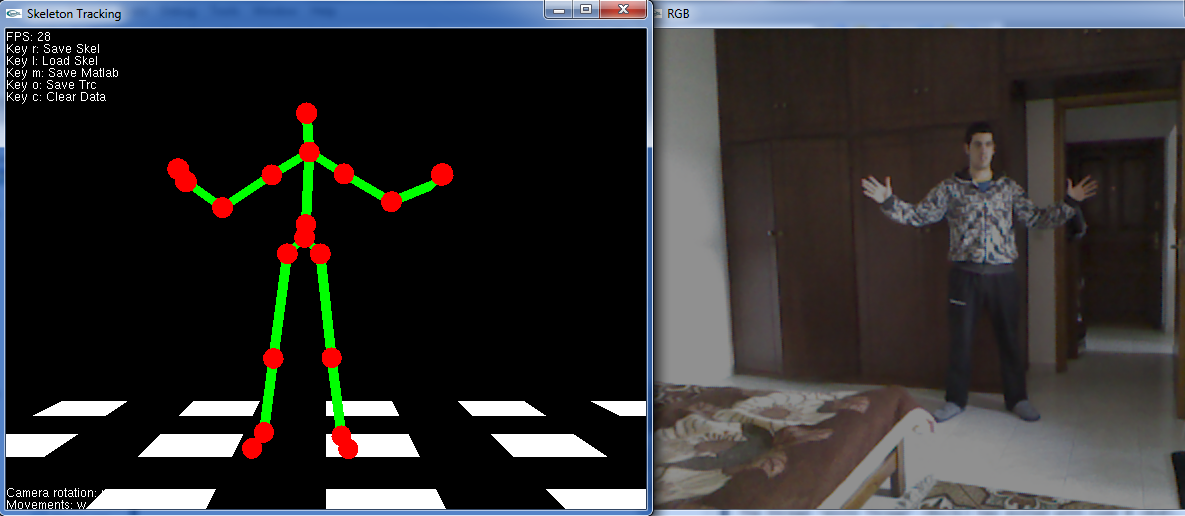
\includegraphics[width=1.0\linewidth, keepaspectratio]{fig/motion-capture.png}
    \end{figure}
    }

    \only<2>{
    \begin{figure}[t]
        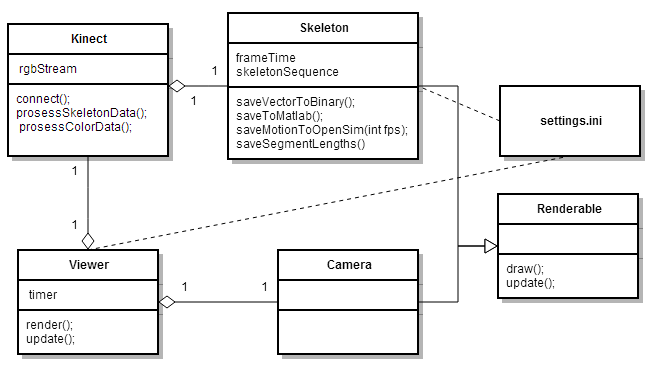
\includegraphics[width=1.0\linewidth, keepaspectratio]{fig/motion-capture-class-diagram.png}
    \end{figure}
    }

\end{frame}

%%%%%%%%%%%%%%%%%%%%%%%%%%%%%%%%%%%%%%%%%%%%%%%%%%%%%%%%%%%%%%%%%%%%%%%%%%%%%%%%
\section{Υλικά και Μέθοδοι}
\frame{\tableofcontents[currentsection]}

\subsection{Περιγραφή της Διαδικασίας}
\begin{frame}
\frametitle{Στάδια της ανάλυσης}

    \only<1>{
    \begin{figure}[t]
        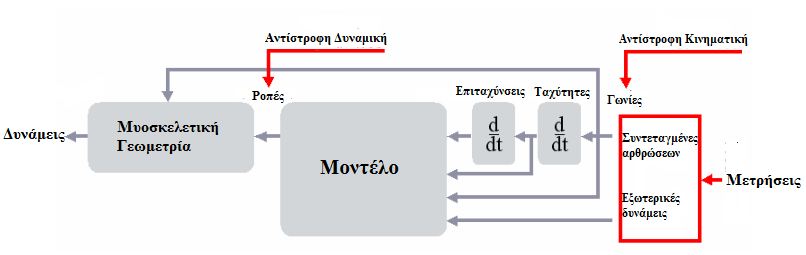
\includegraphics[width=1.0\linewidth, keepaspectratio]{fig/process.png}
    \end{figure}
    }

    \only<2>{
    \begin{figure}[t]
        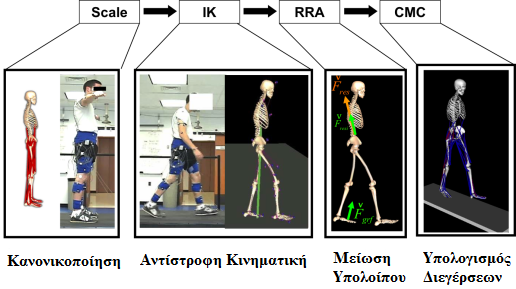
\includegraphics[width=1.0\linewidth, keepaspectratio]{fig/ik-to-excitation.png}
    \end{figure}
    }

    \onslide<1->\let\thefootnote\relax\footnote{\hspace{-12pt}\eng{\url{http://simtk-confluence.stanford.edu:8080/display/OpenSim/Overview+of+the+OpenSim+Workflow}}}

\end{frame}

\subsection{Το Μοντέλο}
\begin{frame}
\frametitle{Περιγραφή του μοντέλου}

    \begin{columns}
        \column{0.4\textwidth}
        \begin{figure}[t]
            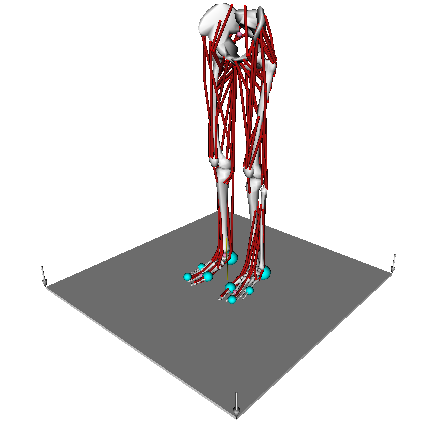
\includegraphics[width=1.0\linewidth, keepaspectratio]{fig/lower-limb-model.png}
        \end{figure}

        \pause

        \column{0.6\textwidth}
        \begin{tabular}{ccc}
            \toprule
            % after \\: \hline or \cline{col1-col2} \cline{col3-col4} ...
            Άρθρωση & Κάτω όριο & Πάνω όριο\\
            \midrule
            \eng{pelvis\_till (z)} & $-90^{o}$ & $+90^{o}$\\
            \eng{pelvis\_list (x)} & $-90^{o}$ & $+90^{o}$\\
            \eng{pelvis\_rotation (y)} & $-90^{o}$ & $+90^{o}$\\
            \eng{pelvis\_tx} & $-5$ & $+5$\\
            \eng{pelvis\_ty} & $-1$ & $+2$\\
            \eng{pelvis\_tz} & $-3$ & $+3$\\
            \eng{hip\_flexion} & $-95^{o}$ & $+95^{o}$\\
            \eng{hip\_adduction} & $-50^{o}$ & $+15^{o}$\\
            \eng{hip\_rotation} & $-20^{o}$ & $+20^{o}$\\
            \eng{knee\_angle} & $-120^{o}$ & $+0^{o}$\\
            \eng{ankle\_angle} & $-30^{o}$ & $+30^{o}$\\
            \eng{subtalar\_angle} & $-20^{o}$ & $+20^{o}$\\
            \eng{mtp\_angle} & $-30^{o}$ & $+30^{o}$\\
            \bottomrule
        \end{tabular}
    \end{columns}

\end{frame}

\subsection{Αντίστροφη Κινηματική}
\begin{frame}
\frametitle{Αντίστροφη κινηματική}

    \begin{block}{Ορισμός}
        Είναι η διαδικασία που μετατρέπει τις θέσεις των αρθρώσεων από το καρτεσιανό τρισδιάστατο χώρο σε γενικευμένες συντεταγμένες του μοντέλου (γωνίες), έτσι ώστε κάθε χρονική στιγμή το μοντέλο να είναι στην ίδια διάταξη με τις μετρήσιμες θέσεις των αντίστοιχων αρθρώσεων.
    \end{block}

    \pause

    \begin{equation*}
        \begin{aligned}
            & \underset{q}{\text{\eng{minimize}}}
            & & \sum_{j=1}^{N} w_{j} \cdot \norm{p_{j} - p(q_{j})}^{2} \\
            & \text{\eng{s.t.}}
            & & c_{j}(q_{j}) \leq b_{j}, \; i = 1, \ldots, N.
        \end{aligned}
    \end{equation*}

\end{frame}

\subsubsection{Τοποθέτηση Ενδείξεων}
\begin{frame}
\frametitle{Τοποθέτηση ενδείξεων}

    \begin{figure}[t]
        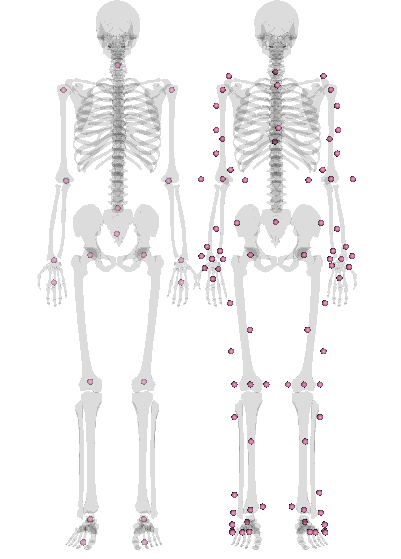
\includegraphics[height=0.9\textheight, keepaspectratio]{fig/kinect-vicon-markers.png}
    \end{figure}

\end{frame}

\subsubsection{Κανονικοποίησης του Μοντέλου}
\begin{frame}
\frametitle{Κανονικοποίησης του μοντέλου}

    \begin{figure}[t]
        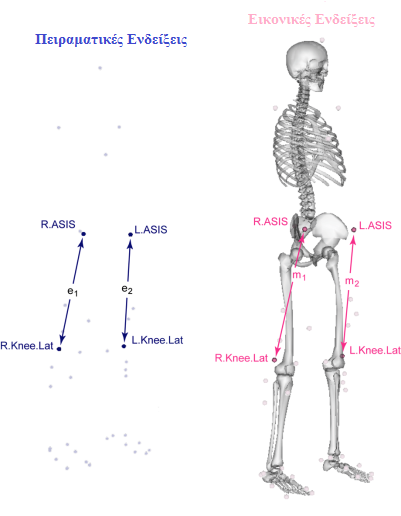
\includegraphics[height=0.8\textheight, keepaspectratio]{fig/scaling.png}
    \end{figure}

    \onslide<1->\let\thefootnote\relax\footnote{\hspace{-12pt}\eng{\url{http://simtk-confluence.stanford.edu:8080/display/OpenSim/How+Scaling+Works}}}

\end{frame}

\subsection{Αντίστροφη Δυναμική}
\begin{frame}
\frametitle{Αντίστροφη δυναμική}

    \begin{block}{Ορισμός}
           Είναι η έρευνα των γενικευμένων ροπών ή δυνάμεων που πρέπει να ασκηθούν στις αρθρώσεις, ώστε το σύστημα να παράξει την συγκεκριμένη κίνηση.
    \end{block}

    \pause

    \begin{equation*}
        M(q) \cdot \ddot{q} + V(q, \dot{q}) + G(q) + F(q, \dot{q}) = \tau
    \end{equation*}

    \pause

    \begin{center}
        \alert{Απαιτείται η γνώση εξωτερικών δυνάμενων}
    \end{center}

\end{frame}

\subsection{Υπολογισμός Μυϊκών Διεγέρσεων}
\begin{frame}
\frametitle{Υπολογισμός μυϊκών διεγέρσεων}

    \begin{figure}[t]
        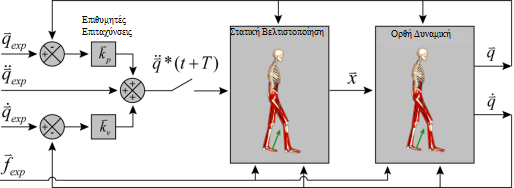
\includegraphics[width=0.9\linewidth, keepaspectratio]{fig/cmc-diagram.png}
    \end{figure}

    \pause

    \begin{equation*}
        \overrightarrow{k}_v = 2 \cdot \sqrt{\overrightarrow{k}_p}
    \end{equation*}

    \pause

    \begin{equation*}
        \begin{gathered}
            \underset{a}{\text{\eng{minimize}}} \sum_{i=1}^{N} a_{i}^{p} \\
            \text{\eng{s.t.}} \quad
            \sum_{i=1}^{N} (a_{i} \cdot f(f^{o}_{i}, l_{i}, v_{i})) \cdot  R_{ij} = \tau_{j}, \quad \forall j
        \end{gathered}
    \end{equation*}

    \onslide<1->\let\thefootnote\relax\footnote{\hspace{-12pt}\eng{Thelen D., "Using computed muscle control to generate forward dynamic simulations of human walking from experimental data", 2006}}

\end{frame}

\subsection{Ορθή Δυναμική}
\begin{frame}
\frametitle{Ορθή δυναμική}

    \only<1>{
    \begin{figure}[t]
        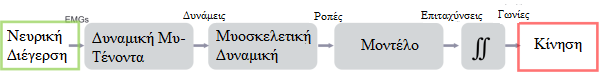
\includegraphics[width=0.9\linewidth, keepaspectratio]{fig/forward-simulation.png}
    \end{figure}

    \begin{equation*}
        \ddot{q} = M(q)^{-1} \cdot \{ \tau - V(q, \dot{q}) - G(q) - F(q, \dot{q})\}
    \end{equation*}
    }

    \only<2>{
    \begin{figure}[t]
        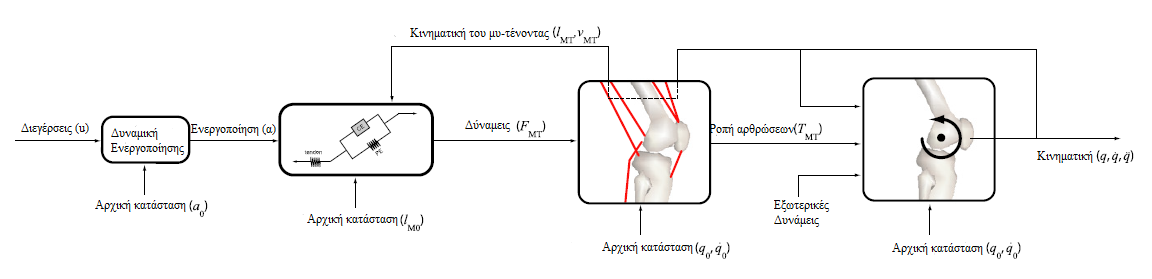
\includegraphics[width=1.0\linewidth, keepaspectratio]{fig/muscle-excitation-force.png}
    \end{figure}

    \begin{equation*}
        \begin{aligned}
            \ddot{q} = M(q)^{-1} \cdot \{ R(q) \cdot F^{M} - V(q, \dot{q}) - G(q) - F(q, \dot{q})\} \\
             f^{M} = f^{M}_{o} \cdot (a \cdot f^{L}(\tilde{l}^{M}) \cdot f^{V}(\tilde{v}^{M}) + f^{PE}(\tilde{l}^{M}))
        \end{aligned}
    \end{equation*}
    }

    \onslide<1->\let\thefootnote\relax\footnote{\hspace{-12pt}\eng{Erdemir A., "Model-based estimation of muscle forces exerted during movements", 2007}}

\end{frame}

%%%%%%%%%%%%%%%%%%%%%%%%%%%%%%%%%%%%%%%%%%%%%%%%%%%%%%%%%%%%%%%%%%%%%%%%%%%%%%%%
\section{Αποτελέσματα}
\frame{\tableofcontents[currentsection]}

\subsection{Σύστημα Καταγραφής}
\begin{frame}
\frametitle{Μορφομετρικά Χαρακτηριστικά}

    \only<1>{
    \begin{figure}[t]
        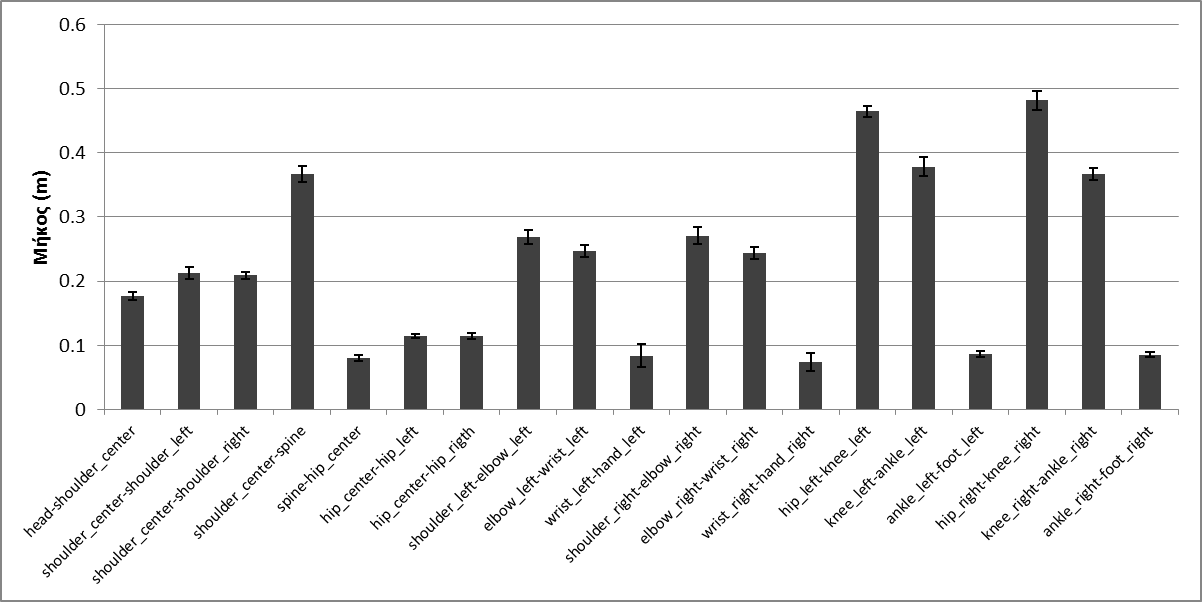
\includegraphics[width=1.0\linewidth, keepaspectratio]{fig/subject01-segments.png}
    \end{figure}

    \begin{center}
        \alert<1>{$std_{min} = 0.0030m, std_{max} = 0.0182m$}
    \end{center}
    }

    \only<2>{
    \begin{figure}[t]
        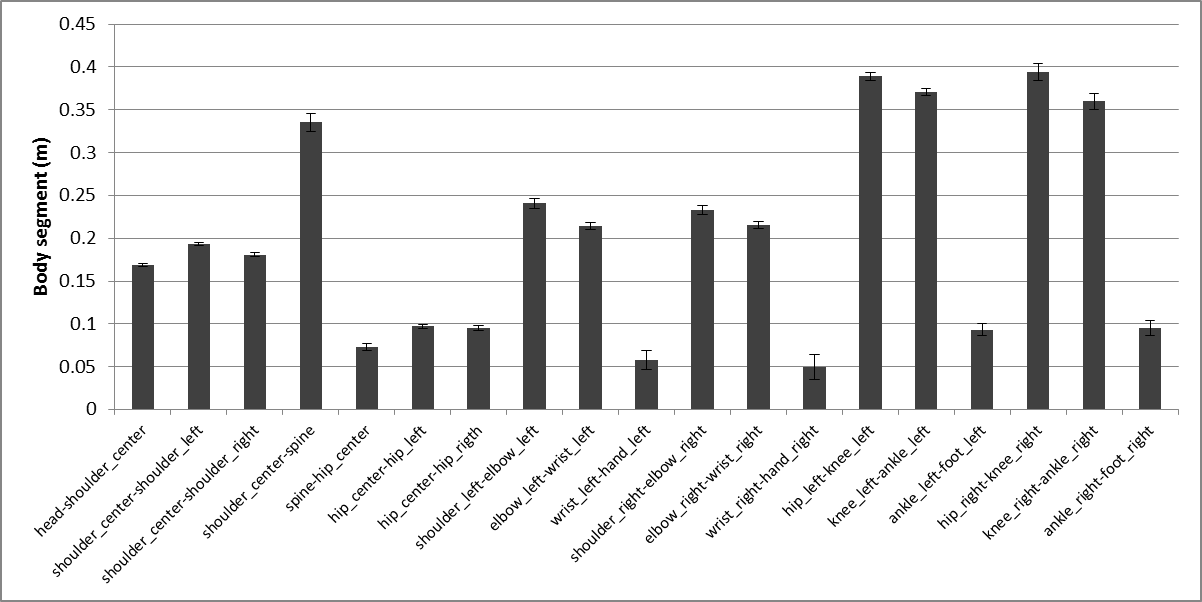
\includegraphics[width=1.0\linewidth, keepaspectratio]{fig/subject02-segments.png}
    \end{figure}

    \begin{center}
        \alert<2>{$std_{min} = 0.0.0019m, std_{max} = 0.0146m$}
    \end{center}
    }

\end{frame}

\begin{frame}
\frametitle{Φιλτράρισμα}

    \begin{columns}
        \column{0.5\textwidth}
        \begin{tabular}{cc}
            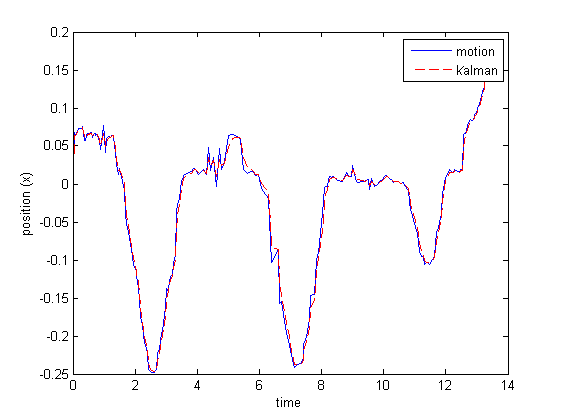
\includegraphics[height = 0.23\textheight, keepaspectratio]{fig/filter0-x.png} & 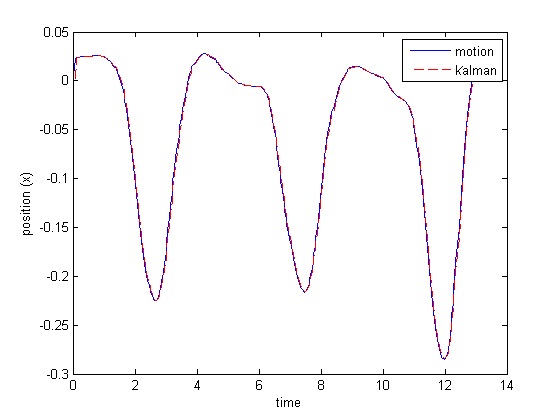
\includegraphics[height = 0.23\textheight, keepaspectratio]{fig/filter3-x.png}\\
            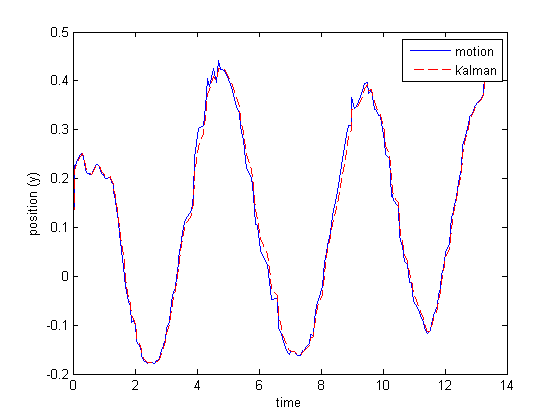
\includegraphics[height = 0.23\textheight, keepaspectratio]{fig/filter0-y.png} & 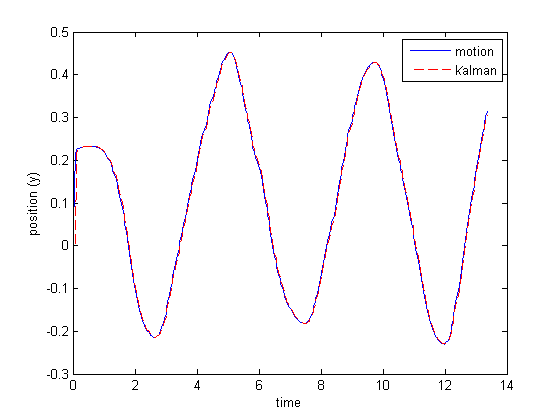
\includegraphics[height = 0.23\textheight, keepaspectratio]{fig/filter3-y.png}\\
            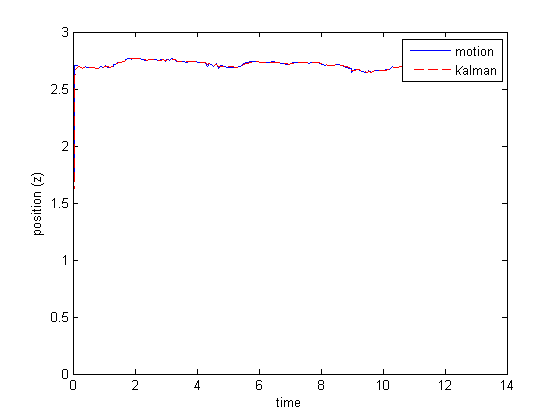
\includegraphics[height = 0.23\textheight, keepaspectratio]{fig/filter0-z.png} & 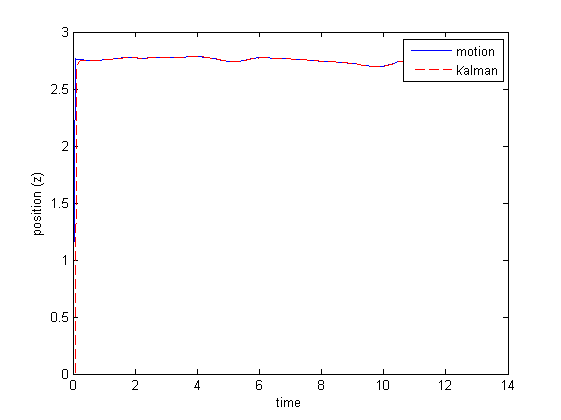
\includegraphics[height = 0.23\textheight, keepaspectratio]{fig/filter3-z.png}\\
            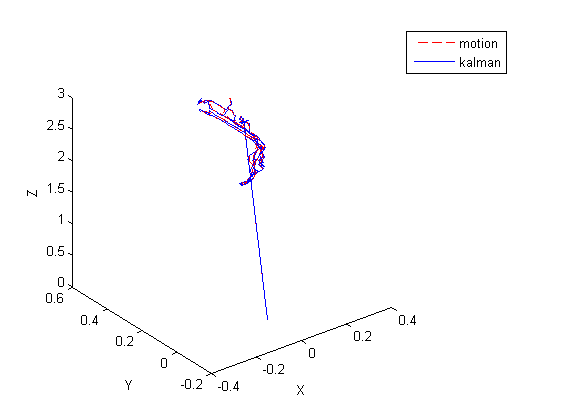
\includegraphics[height = 0.23\textheight, keepaspectratio]{fig/filter0-xyz.png} & 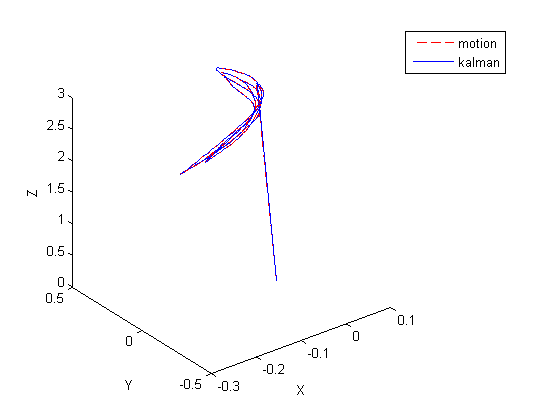
\includegraphics[height = 0.23\textheight, keepaspectratio]{fig/filter3-xyz.png}
        \end{tabular}

        \pause

        \column{0.5\textwidth}
        \begin{equation*}
            \begin{gathered}
                \text{Πρόβλεψη} \\
                \hat{p}_{t} = p_{t-1} + u_{t}, \quad u_{t} = \frac{p_{t-1} - p_{t-2}}{t_{t-1} - t_{t-2}} \\
                \hat{P} = P_{t-1} + Q \\[.5cm]
                \text{Διόρθωση} \\
                Κ = \frac{\hat{P}}{\hat{P} + R}\\
                p_{t} = \hat{p}_{t} + K \cdot (p_{t} - \hat{p}_{t}) \\
                P_{t} = (1 - K) \cdot \hat{P}
            \end{gathered}
        \end{equation*}

        \begin{center}
            \href{run:video/filter0.avi}{
\includegraphics[scale=0.15]{fig/play.jpeg}}
            \href{run:video/filter3.avi}{
\includegraphics[scale=0.15]{fig/play.jpeg}}
        \end{center}

    \end{columns}

\end{frame}

\begin{frame}
\frametitle{Αντίστροφη κινηματική}

    \only<1>{
    \begin{center}
        \begin{tabular}{cc}
            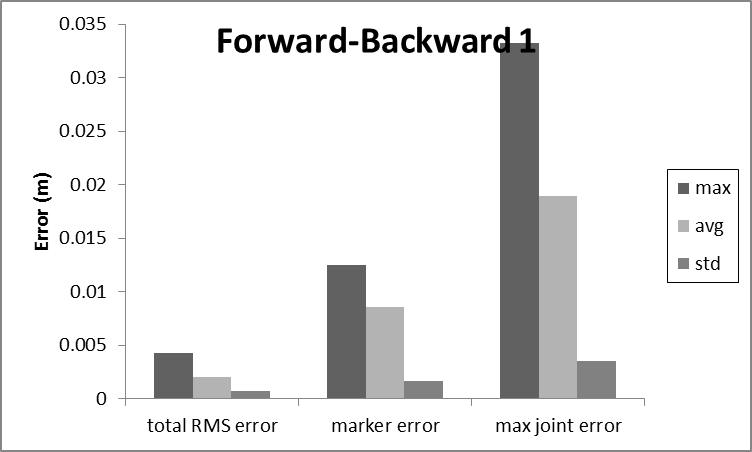
\includegraphics[width=.48\textwidth, height = 0.25\textheight, keepaspectratio]{fig/ik-reg1.png} & 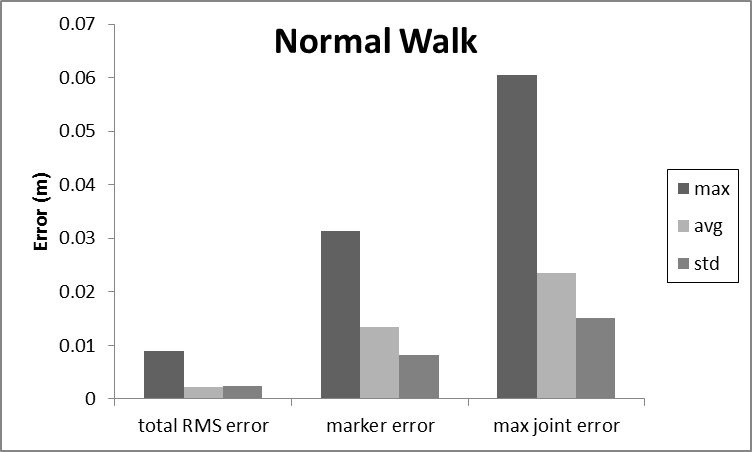
\includegraphics[width=.48\textwidth, height = 0.25\textheight, keepaspectratio]{fig/ik-reg2.png}\\[3pt]
            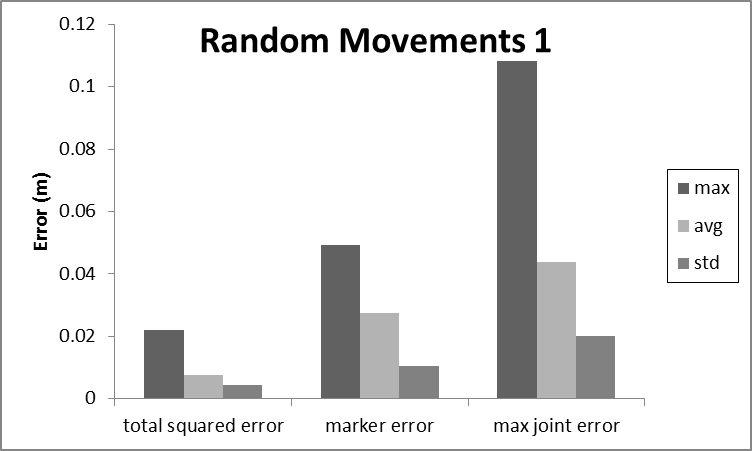
\includegraphics[width=.48\textwidth, height = 0.25\textheight, keepaspectratio]{fig/ik-reg3.png} & 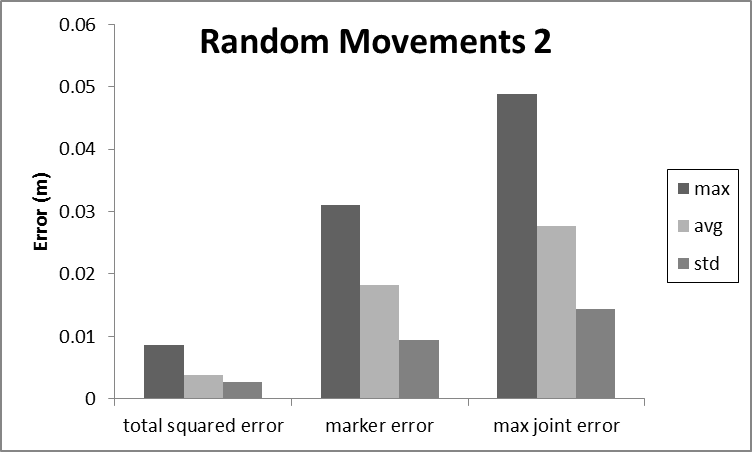
\includegraphics[width=.48\textwidth, height = 0.25\textheight, keepaspectratio]{fig/ik-reg4.png}\\[3pt]
            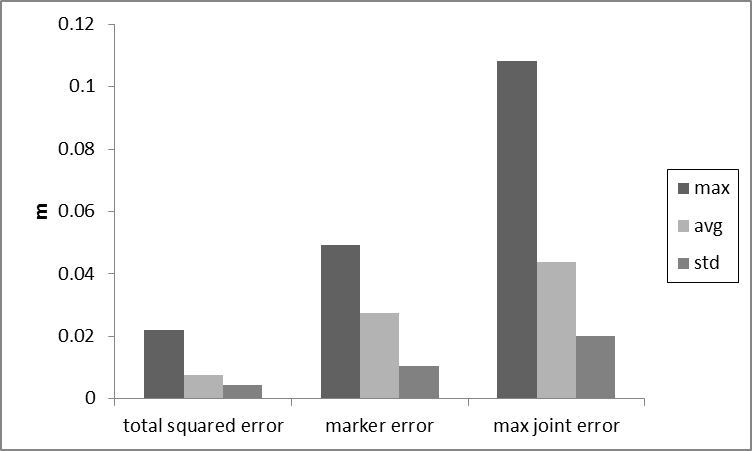
\includegraphics[width=.48\textwidth, height = 0.25\textheight, keepaspectratio]{fig/ik-reg5.png} & 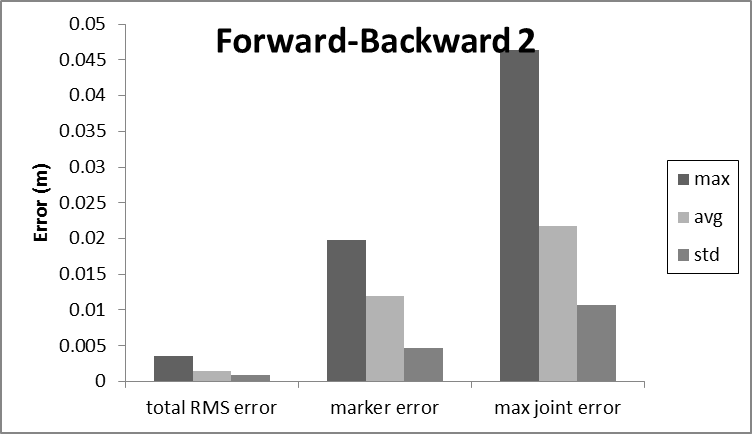
\includegraphics[width=.48\textwidth, height = 0.25\textheight, keepaspectratio]{fig/ik-reg6.png}
        \end{tabular}
    \end{center}
    }

    \only<2-3>{
    \begin{figure}[c]
        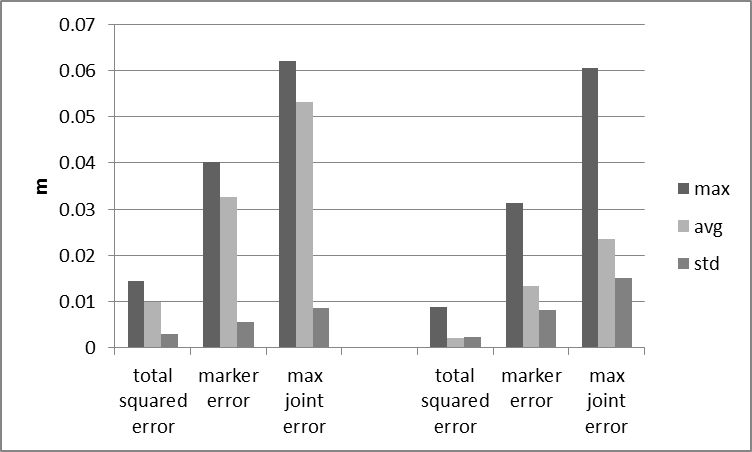
\includegraphics[width=1.0\linewidth, keepaspectratio]{fig/ik-no-scale-with-scale.png}
    \end{figure}
    
    \begin{center}
        \href{run:video/walk-motion-capture.avi}{
\includegraphics[scale=0.15]{fig/play.jpeg}}
        \href{run:video/walk-opensim.avi}{
\includegraphics[scale=0.15]{fig/play.jpeg}}
    \end{center}
    }

\end{frame}

\subsection{Δυναμική Ανάλυση}
\begin{frame}
\frametitle{Αντίστροφη δυναμική}

    \begin{center}
        \begin{tabular}{cc}
            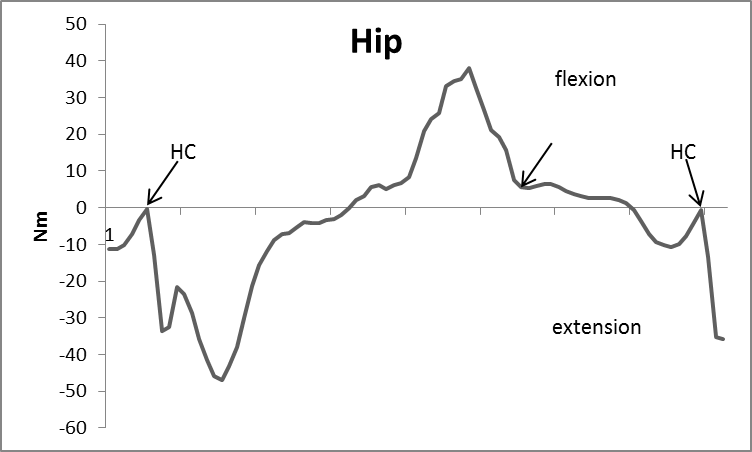
\includegraphics[width=.48\textwidth, height = 0.25\textheight, keepaspectratio]{fig/id-hip.png} & 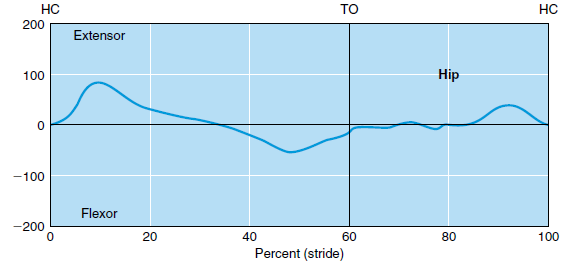
\includegraphics[width=.48\textwidth, height = 0.25\textheight, keepaspectratio]{fig/id-hip-ref.png}\\[3pt]
            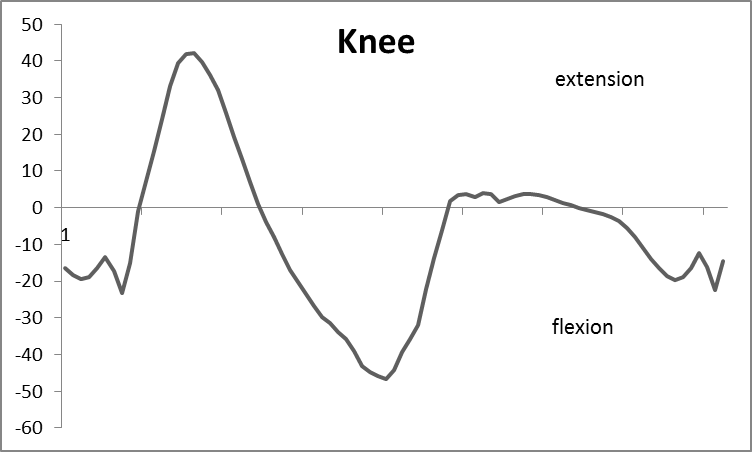
\includegraphics[width=.48\textwidth, height = 0.25\textheight, keepaspectratio]{fig/id-knee.png} & 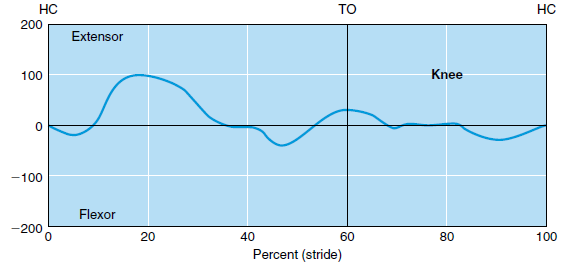
\includegraphics[width=.48\textwidth, height = 0.25\textheight, keepaspectratio]{fig/id-knee-ref.png}\\[3pt]
            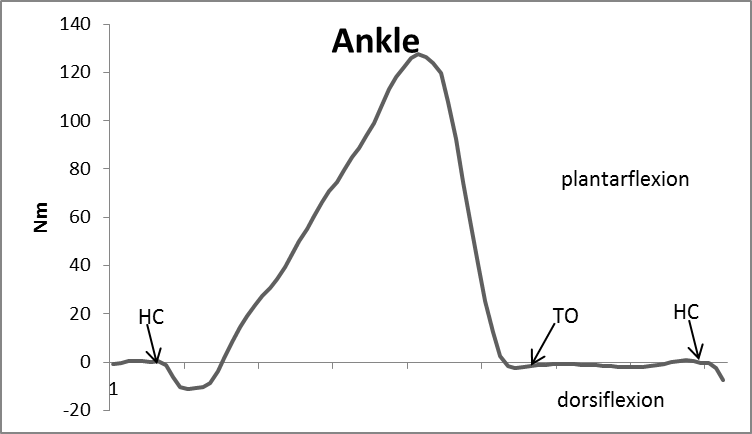
\includegraphics[width=.48\textwidth, height = 0.25\textheight, keepaspectratio]{fig/id-ankle.png} & 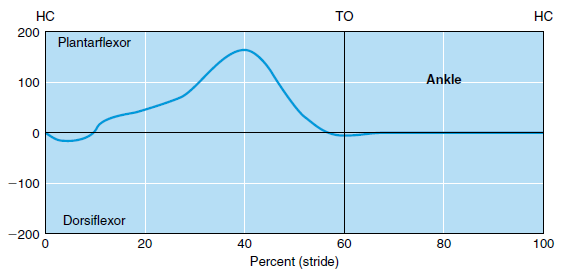
\includegraphics[width=.48\textwidth, height = 0.25\textheight, keepaspectratio]{fig/id-ankle-ref.png}
        \end{tabular}
    \end{center}

    \onslide<1->\let\thefootnote\relax\footnote{\hspace{-12pt}\eng{Whittlesey Saunders, Robertson Gordon, "Two-Dimention Inverse Dynamics"}}

\end{frame}

\begin{frame}
\frametitle{Ορθή Δυναμική}

    \begin{tabular}{cc}
        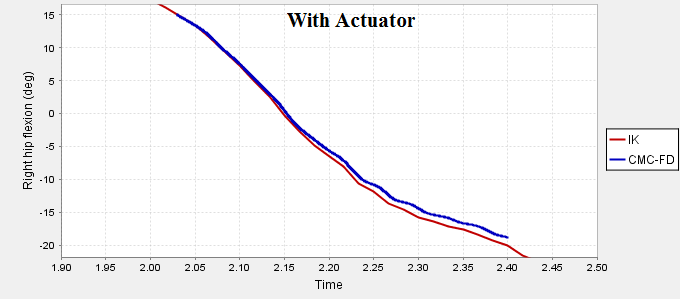
\includegraphics[width=.48\textwidth, keepaspectratio]{fig/hip-ik-cmc.png} & \includegraphics[width=.48\textwidth, keepaspectratio]{fig/hip-ik-id.png}\\[3pt]
        \includegraphics[width=.48\textwidth, keepaspectratio]{fig/knee-ik-cmc.png} & \includegraphics[width=.48\textwidth, keepaspectratio]{fig/knee-ik-id.png}\\[3pt]
        \includegraphics[width=.48\textwidth, keepaspectratio]{fig/ankle-ik-cmc.png} & \includegraphics[width=.48\textwidth, keepaspectratio]{fig/ankle-ik-id.png}
    \end{tabular}

\end{frame}

\end{document} 